\documentclass{article}
\usepackage[a4paper, landscape, left=1cm, right=1cm, top=1.7cm, bottom=1.2cm]{geometry}
\usepackage[utf8]{inputenc}
\usepackage[english]{babel}

\usepackage{multicol}
\usepackage{amssymb}
\usepackage{amsmath}
\usepackage{mathtools}
\usepackage{cancel}

\usepackage{graphicx}

\usepackage{enumitem}
\setlist[enumerate]{label*=\arabic*.}

\usepackage{listings}
\usepackage{color}

\definecolor{dkgreen}{rgb}{0,0.6,0}
\definecolor{gray}{rgb}{0.5,0.5,0.5}
\definecolor{mauve}{rgb}{0.58,0,0.82}

\lstset{frame=tb,
  language=Python,
  aboveskip=3mm,
  belowskip=3mm,
  showstringspaces=false,
  columns=flexible,
  basicstyle={\small\ttfamily},
  numbers=none,
  numberstyle=\tiny\color{gray},
  keywordstyle=\color{blue},
  commentstyle=\color{dkgreen},
  stringstyle=\color{mauve},
  breaklines=true,
  breakatwhitespace=true,
  tabsize=3
}

% change list spacing
\usepackage{enumitem}
\setlist[1]{itemsep=-3pt}

%set header spacing


\usepackage[compact]{titlesec}
\titlespacing{\section}{0pt}{*0}{*0}
\titlespacing{\subsection}{0pt}{*0}{*0}
\titlespacing{\subsubsection}{0pt}{*0}{*0}



% declare delimiter for ceil and floor from mathtools
\DeclarePairedDelimiter\ceil{\lceil}{\rceil}
\DeclarePairedDelimiter\floor{\lfloor}{\rfloor}

% remove indentaion
\setlength\parindent{0pt}

\usepackage{fancyhdr} % to change header and footers

% inline code
\NewDocumentCommand{\codeword}{v}{%
\texttt{\textcolor{blue}{#1}}%
}

\pagestyle{fancy} % Turn on the style
\fancyhf{} % Start with clearing everything in the header and footer
% Set the right side of the footer to be the page number
\fancyfoot[R]{\thepage}

% Redefine plain style, which is used for titlepage and chapter beginnings
% From https://tex.stackexchange.com/a/30230/828
\fancypagestyle{plain}{%
    \renewcommand{\headrulewidth}{0pt}%
    \fancyhf{}%
    \fancyfoot[R]{\thepage}%
}

% solve > becoming weird
\usepackage{lmodern}

\rhead{Chang CH}
\lhead{CS3223 Cheatsheet}
\rfoot{Page \thepage}

\setlength{\columnseprule}{0.1pt}


\begin{document}
\begin{multicols*}{4}

\section{Hardware}
\subsection{Disk Access time}
\begin{itemize}
  \item Disk access time: seek + rotational + transfer
  \item seek time: move arms to correct track. 5-6ms fixed
  \item rotational delay: rotate track to correct block. avg  $1/2$ round 
\end{itemize}

\subsection{DB terminology}
\begin{itemize}
  \item Buffer pool: cache. split into frames, each frame same size as blocks.
  \item Frames: store pin count (no. clients using) + dirty flag(modified but not in disk)
  \item Disk blocks: aka pages. unit of retrieval, consist of contiguous sectors.
  \item Clock replacement: if pin count == 0: if referenced bit off evict else turn referenced bit off. Does not reset after an op.
  \item notation: $|A|$ number of pages to store A, $||A||$ number of records in A.
\end{itemize}

\subsection{File implementation}
Each record has an id called RID (page id + slot number). 1 page many slots.
\begin{enumerate}
  \item Heap file, unordered. page header store 2 linked list of pages. 1 linked list free space, 1 used.
  \item Sorted file, ordered by search key
  \item Hashed file, locate block by hash function.
\end{enumerate}
Record organization in pages
\begin{enumerate}
  \item fixed, packed: store records in contiguous slots. header store number of records
  \item fixed, unpacked: use bit array to indicate if slot if full, can choose any slots.
  \item variable length
\end{enumerate}
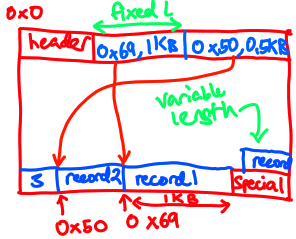
\includegraphics[width=\linewidth]{./res/pgSlottedPage.png}

\section{Indexes}
Data structures to speed up info retrieval. search key = sequence of attributes. unique index = search key is candidate key.

\subsection{B+ tree}
formats:
\begin{enumerate}
  \item key, actual record
  \item key, record id
  \item key, array of record ids
\end{enumerate}
notes:
\begin{itemize}
  \item internal node, < lhs, $\geq$ rhs
  \item non leaf nodes are not values: $5 \rightarrow [4][7]$, 5 does not exist as record
  \item order \codeword{d} b+ tree: nodes contain at least \codeword{d} nodes, at most \codeword{2d} nodes
  \item No dupes. irl usually take some unique attrib also.
  \item clustered index: sort order of index is same as table. e.g. sort on weight, weight 1,2,3 on same data page. (at most 1 clustered index since actual data must sort 1 way.)
  \item dense index: index record (key + pointer) exists for every search key value. (therefore format 2,3 sure dense)
\end{itemize}

\subsubsection{Insert}
\begin{enumerate}
  \item if page not full, insert.
  \item check right neighbor (must same parent) then left
  \item if not full, redistribute (largest record go over, update internal node)
  \item split page. order \codeword{d} table, \codeword{d} records in original page, \codeword{d+1} in new page. add entry in internal node.
  \item if internal node full, repeat steps above for internal. internal node split, promote middle node 1 level.
\end{enumerate}

\subsubsection{Delete}
same as insert. check right then left. redistribute if neighbor size > \codeword{d}. Merge if cannot (delete internal node between).

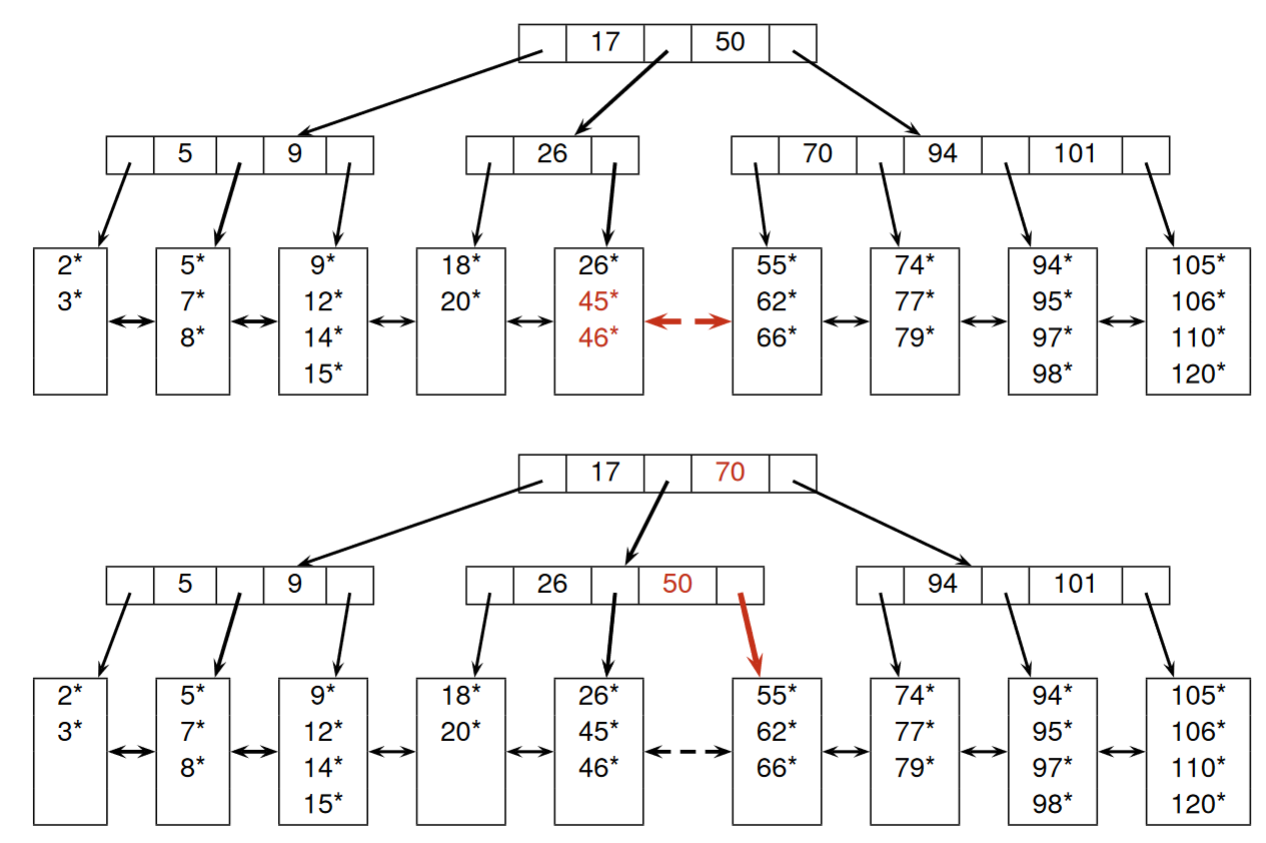
\includegraphics[width=\linewidth]{./res/bredist.png}

\subsubsection{Bulk loading}
\begin{enumerate}
  \item sort records, pack into pages of \codeword{2d} records
  \item keep inserting, add internal node record each time. split if need be.
\end{enumerate}

\subsection{Hashed based}
static hashing: \codeword{N} buckets, hash is simple modulo. linked list of overflow data pages.

\subsubsection{Linear hashing}
\codeword{N}: number of buckets. \codeword{next}: next bucket to split. $N_\mathrm{level}$: number of pages at level. starts at 0. 
bucket index starts at 0. 
Only split when a page overflows. If overflow page not full do not split.
\begin{enumerate}
  \item Check if bucket \codeword{j} to insert to is full. Insert if not.
  \item \codeword{next} is not \codeword{j}, split bucket \codeword{next}. \codeword{next++}. insert page into overflow page.
  \item if \codeword{next} is \codeword{j}, split bucket. \codeword{next++}. If bucket to insert into is still full, insert into overflow page.
  \item if \codeword{next} is $N_\mathrm{level}$ during split, set \codeword{next} to 0, \codeword{level++}. $N_\mathrm{level} = 2^\mathrm{level} - 1$.
\end{enumerate}
To cause max splits, insert numbers such that after split, 1 bucket just nice full. Deletion, if last bucket empty, delete and decrement next if next > 0, else decrement level.

\subsubsection{Extendible hashing}
like linear hashing, except keep directory of pointers to buckets.
\begin{enumerate}
  \item Insert \codeword{01}. no overflow ok.
  \item overflow, double directory size. \codeword{001}, \codeword{101} point to separate buckets
  \item other keys e.g. \codeword{000}, \codeword{100} done need new bucket, point to original \codeword{00} bucket.
\end{enumerate}
note: last bucket of split must contain bucket size + 1 items. possible that 4 pointer to same bucket split into 2 buckets with 2 pointers each.

\section{sort select}
\subsection{external sorting}
\begin{itemize}
  \item External sorting of \codeword{x} data pages using \codeword{m} buffer/memory pages (x >> \codeword{m})
  \begin{enumerate}
    \item Create sorted runs, each run size \codeword{m}. page cost: $2 * x$.
    \item Merge runs \codeword{m - 1} ways. 1 output page rest input. 
    \item Selection sort, write to disk when output full. page cost = $2 * x * depth$.
  \end{enumerate}
  
  \item optimization, blocked I/O
  \begin{itemize}
    \item system sometimes allow reading of \codeword{b} contiguous pages in 1 i/o operation (same seek + rotational, longer transfer)
    \item io time: instead of $x * pageRWtime$ use $blocks * blockRWtime$ each pass. initial pass take block size as buffer size.
  \end{itemize}
\end{itemize}

\subsection{B+ tree sort select}
\begin{itemize}
  \item selectivity og access path: no. of index/data pages needed to get record. smallest usually = traverse down smallest value, iterate right.
  \item covering index for \codeword{Q}: index contains all info required, no need fetch with RID etc.
  \item \codeword{where ... and}: look up RID and filter or intersect with another b+ tree index.
\end{itemize}

\subsubsection{conjuncts}
\begin{itemize}
  \item Conjunctive Normal Form: express in ands. conjuncts = \codeword{A or B}.
  \item index \codeword{K(k1, ... kn)} matches predicate \codeword{p} if:
  \begin{itemize}
    \item b+ tree: \codeword{p} is of the form \codeword{(k1 = c1) && ...(Ki = ci) && (Kj op cj)}. At most 1 non \codeword{==} op, must be last attrib. does not have to be all of index.
    \item hash index: like b+ but no non \codeword{==} + all attributes used (kb = cn).
  \end{itemize}
  \item \codeword{where ... and}: look up RID and filter or intersect with another b+ tree index.
  \item primary conjuncts: subset of conjuncts in \codeword{p} that index \textbf{matches}.
  \item covered conjuncts: conjuncts in \codeword{p} that index covers. conjuncts may not be primary (see matches def.)
\end{itemize}

\subsubsection{cost}
\begin{itemize}
  \item b+ tree: pages accessed = leaf depth + no leaf pages to scan. if format 2/3, + no. of entries(need lookup each)
  \item hash: scan leaf pages(num entries to get / num entries per leaf page)
  \item if index is covering, no need RID lookup even if format 2/3.
\end{itemize}
best query plan: consider table scan, index scan, index intersection.
\section{projection}
Pick subset of attributes then dedupe. project with * mean no dedupe.
\subsubsection{sort based}
\begin{enumerate}
  \item extract all columns needed. cost = \codeword{R} read num pages original + \codeword{T} write num pages intermediate table.
  \item sort all column \codeword{2 * T * depth}. depth inclusive initial sorted.
  \item scan and dedupe, read \codeword{T} write omitted (return).
  \item optimization: create initial sorted runs at step 1, dedupe during merge. no dedupe cost, merge depth exclude initial.
  \item if exists index (preferably covering/clustered) can use also try index scan. if unclustered, for each tuple need RID lookup so very expensive. clustered can scan by pages for same sort key.
  \item if index only partial, can use values with same sort key as partition, project within partition.
\end{enumerate}

\section{joins}
Outer join Inner, R join S. can swap R and S.
\subsubsection{iteration}
\begin{enumerate}
  \item For each record in outer (cost = $|R|$)
  \item scan each record in inner. cost = $||R|| * |S|$ (can optimize for each page $|R|$)
  \item block nested, 1 output 1 \codeword{S}, rest \codeword{R}. cost = $|R| / (B - 2) *  |S|$
\end{enumerate}
\subsubsection{Sort merge join}
\begin{enumerate}
  \item sort inner + outer
  \item join. may need rewind if dupes: R = 10,10,20 S = 10, 10, 15. cost = $|R| + |S|$
  \item if $|buffer|$ > \# initial runs \codeword{R} \& \codeword{S}, after initial sorted run can join already.
\end{enumerate}

\subsubsection{Hash join}
\begin{enumerate}
  \item hash inner, outer into \codeword{k} partitions each
  \item say inner.A = 1 in partition 1 and outer.A = 1 in partition 3, join partition 1 + 3.
  \item 1 output 1 input, rest use as hash table for inner. probe outer into input, write to output. output full write to disk.
  \item cost: $3 * (numPagesInner + numPagesOuter)$. 
  \item $k = B - 1$, $B \approx \sqrt[2]{f * numPagesInner}$, \codeword{f} is fudge factor.
\end{enumerate}


\end{multicols*}
\end{document}
